\documentclass{jlreq}

\usepackage{titlesec}
\usepackage{listings}
\usepackage{fancyhdr}

% \adjustbox
\usepackage{adjustbox}

% tcolorboxの設定
\usepackage[most]{tcolorbox} 
\tcbuselibrary{breakable}
\tcbuselibrary{skins}
\tcbuselibrary{listingsutf8}
% タイトルのフォーマットを変更
\titleformat{\title}
  {\centering\Huge\bfseries}
  {}
  {0em} 
  {}

\titleformat{\subtitle}
  {\centering\Large\itshape}
  {}
  {0em}
  {}

\titleformat{\subsubsection}[block]
  {\normalfont\normalsize\bfseries}
  {\arabic{subsubsection}.}
  {1em}
  {}

\titleformat{\section}[block]
  {\normalfont\large\bfseries}
  {\Roman{section}.}
  {1em} 
  {}
  [\titleline{\titlerule[1pt]}]

\titleformat{\subsection}[block]
  {\normalfont\normalsize\bfseries}
  {\roman{subsection}.}
  {1em}
  {}

% listingsの設定

\renewcommand{\lstlistingname}{コード}

\lstset{
	breaklines = true,
	language = Python,
	keywordstyle = {\bfseries \color[cmyk]{0,1,0,0}},
	commentstyle = {\itshape \color[cmyk]{1,0.4,1,0}},
	numbers = left,
	numberstyle = \tiny,
	stepnumber = 1,
	% frameとnumberの間の距離
	numbersep = 10pt,
	frame = single,
	basicstyle = \ttfamily,
	tabsize = 2,
	captionpos = t,
	backgroundcolor={\color[gray]{.90}},
	showstringspaces = false,
}

% headerの設定
\pagestyle{fancy}
\fancyhf{}

\fancyhead[RO,RE]{\rightmark}
\fancyhead[LO,LE]{\leftmark} 
\fancyfoot[C]{\thepage}

% tikzの設定
\usepackage{tikz}

\begin{document}

EEIC2024アルゴリズムの授業で扱ったデータ構造のアルゴリズムのシケプリです。扱った内容は以下の通りです。
\begin{itemize}
	\item スタック
	\item キュー
	\item 線形リスト
	\item ツリー
	\item ヒープ
	\item セグメント木(発展的な内容)
	\item BIT(発展的な内容)
\end{itemize}

\section{スタック}

スタックはLIFO(Last In First Out)といって、最後に入れたデータが最初に取り出されるデータ構造です。本を積み重ねるイメージで考えるとわかりやすいです。スタックには以下の操作があります。

\begin{itemize}
	\item push: スタックにデータを追加する
	\item pop: スタックからデータを取り出す
\end{itemize}

\vspace{1cm}

\begin{center}
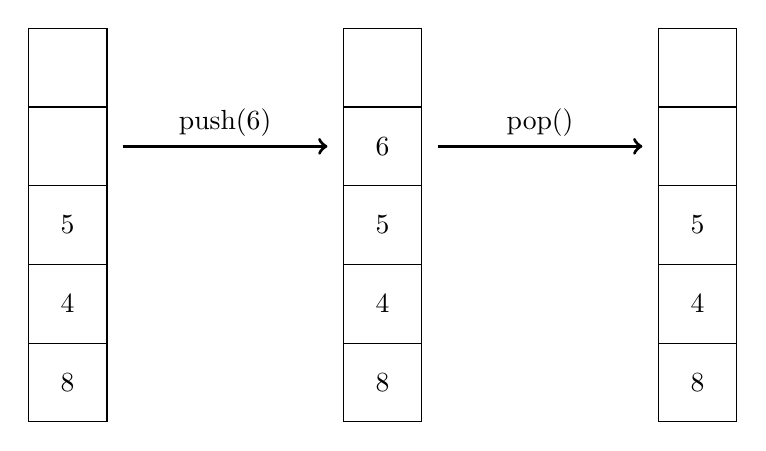
\begin{tikzpicture}
		\draw (0, 0) rectangle (1, 1);
		\node at (0.5, 0.5) {8};
		\draw (0, 1) rectangle (1, 2);
		\node at (0.5, 1.5) {4};
		\draw (0, 2) rectangle (1, 3);
		\node at (0.5, 2.5) {5};
		\draw (0, 3) rectangle (1, 4);
		\draw (0, 4) rectangle (1, 5);
	
		\draw (4, 0) rectangle (5, 1);
		\node at (4.5, 0.5) {8};
		\draw (4, 1) rectangle (5, 2);
		\node at (4.5, 1.5) {4};
		\draw (4, 2) rectangle (5, 3);
		\node at (4.5, 2.5) {5};
		\draw (4, 3) rectangle (5, 4);
		\node at (4.5, 3.5) {6};
		\draw (4, 4) rectangle (5, 5);
	
		\draw (8, 0) rectangle (9, 1);
		\node at (8.5, 0.5) {8};
		\draw (8, 1) rectangle (9, 2);
		\node at (8.5, 1.5) {4};
		\draw (8, 2) rectangle (9, 3);
		\node at (8.5, 2.5) {5};
		\draw (8, 3) rectangle (9, 4);
		\draw (8, 4) rectangle (9, 5);

		% pushと文字を描画
		\draw[->, very thick] (1.2, 3.5) -- (3.8, 3.5);
		\node at (2.5, 3.8) {push(6)};	

		% popと文字を描画
		\draw[->, very thick] (5.2, 3.5) -- (7.8, 3.5);
		\node at (6.5, 3.8) {pop()};
\end{tikzpicture}
\end{center}

\vspace{0.5cm}
\begin{center}
	\textbf{スタックのイメージ}
\end{center}
\vspace{0.5cm}

\subsection{スタックの実装}
実装のポイントは以下の3つです。Pythonのclassを使って実装します。
\begin{itemize}
	\item スタックは配列で実装する
	\item 要素が入る位置を示すポインタを持つ
	\item pushとpopのメソッドを実装する
\end{itemize}

実装は以下の\ref{stack}のようになります。

\begin{lstlisting}[caption=スタックの実装, label=stack, frame=TRBL, label={stack}]
	class Stack:
    def __init__(self, size: int) -> None:
        self.stack: list[int] = [0] * size
        self.top: int = 0
    
    def push(self, value: int) -> None:
        if self.top < len(self.stack):
            self.stack[self.top] = value
            self.top += 1
        else:
            print("This stack is full.")
    
    def pop(self) -> None:
        if self.top > 0:
            self.top -= 1
            return_value = self.stack[self.top]
            return return_value
        else:
            print("This stack is empty.")

def main():
    size = 5
    stack = Stack(size)
    
    stack.push(8)
    stack.push(4)
    stack.push(5)
    stack.push(6)
    return_value = stack.pop()
    
    print(f"returned value is {return_value}")
    
main()

\end{lstlisting}

\begin{tcolorbox}[enhanced, title=Column1 collections.deque, breakable, colback=white, drop fuzzy shadow, attach boxed title to top center={yshift*=0.1cm}]
	実際にスタックを使用するときは、Pythonの標準ライブラリであるcollectionsのdequeを使うと便利です。PythonではStack スタックやキューが明示的に用意されていないため、双方向キューであるdequeを使ってスタックやキューを使用します。
	スタックは上記のように配列で簡単に実装可能ですが、標準ライブラリのdequeを使うことで、より高速にスタックを使用できます。

	\begin{lstlisting}[caption=スタックの実装, label=stack, frame=TRBL, label={stack}]
		def main():
    from collections import deque
    stack = deque()
    
    stack.append(8)
    stack.append(4)
    stack.append(5)
    stack.append(6)
    
    return_value = stack.pop()
    
    print(f"returned value is {return_value}")
    
main()
    	
	\end{lstlisting}
\end{tcolorbox}

\newpage

\section{キュー}
キューはFIFO(First In First Out)といって、最初に入れたデータが最初に取り出されるデータ構造です。ディズニーランドの待ち行列のようなイメージで考えるとわかりやすいです。
キューには以下のような操作があります。

\begin{itemize}
	\item enqueue: キューにデータを追加する
	\item dequeue: キューからデータを取り出す
\end{itemize}

先ほどのスタックと違って配列の頭からデータを取り出していることに注意してください。つまり、dequeueをするたびに
取り出すデータの位置をずらす必要があります。従って、データを取り出すための先頭アドレス、データを追加するための末尾アドレスを持つ必要があります。

しかし、ここで困ったことがあります。dequeueをするたびに配列の頭が右にずれていくと、配列の先頭にデータが残っているにも関わらず、配列の末尾にデータが追加できなくなります。この問題を解決するために、リングバッファ
というデータ構造を使います。

\vspace{1cm}

\begin{center}
	\begin{tikzpicture}
		\draw (0, 0) rectangle (1, 1);
		\node at (0.5, 0.5) {8};
		\draw (1, 0) rectangle (2, 1);
		\node at (1.5, 0.5) {4};
		\draw (2, 0) rectangle (3, 1);
		\node at (2.5, 0.5) {5};
		\draw (3, 0) rectangle (4, 1);
		\draw (4, 0) rectangle (5, 1);

		% enqueueの丸と矢印を描画
		\draw (6.5, 0.5) circle[radius=0.5];
		\draw [<-] (5.2, 0.5) -- (6.0, 0.5);
		\node at (6.5, 0.5) {2};

		\draw (0, -3) rectangle (1, -2);
		\node at (0.5, -2.5) {8};
		\draw (1, -3) rectangle (2, -2);
		\node at (1.5, -2.5) {4};
		\draw (2, -3) rectangle (3, -2);
		\node at (2.5, -2.5) {5};
		\draw (3, -3) rectangle (4, -2);
		\node at (3.5, -2.5) {2};
		\draw (4, -3) rectangle (5, -2);

		% dequeueの丸と矢印を描画
		\draw (-1.0, -2.5) circle[radius=0.5];
		\draw [<-] (-2.5, -2.5) -- (-1.5, -2.5);
		\node at (-1.0, -2.5) {8};

		\draw (0, -6) rectangle (1, -5);
		\draw (1, -6) rectangle (2, -5);
		\node at (1.5, -5.5) {4};
		\draw (2, -6) rectangle (3, -5);
		\node at (2.5, -5.5) {5};	
		\draw (3, -6) rectangle (4, -5);
		\node at (3.5, -5.5) {2};
		\draw (4, -6) rectangle (5, -5);

		% enqueueと文字を描画
		\draw[->, very thick] (2.4, -1.0) -- (2.4, -1.8);
		\node at (2.5, -0.8) {enqueue(2)};

		% dequeueと文字を描画
		\draw[->, very thick] (2.4, -4.0) -- (2.4, -4.8);
		\node at (2.5, -3.8) {dequeue()};

	
	\end{tikzpicture}
\end{center}

\begin{adjustbox}{center}
	% 初期状態:3要素が入っている状態
	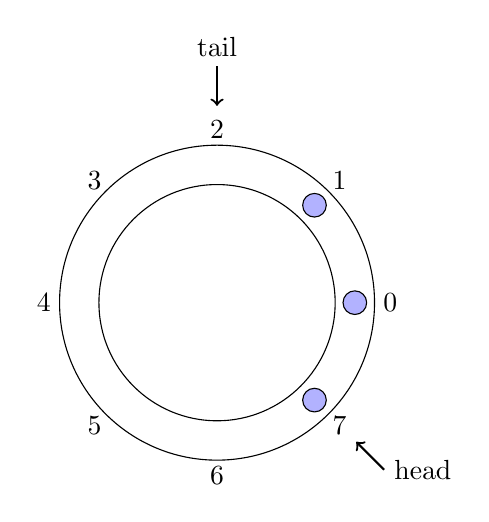
\begin{tikzpicture}
		\draw (0, 0) circle[radius=2];
		\draw (0, 0) circle[radius=1.5];
	
		\foreach \i in {0, 1, 2, 3, 4, 5, 6, 7} {
			\node at ({360/8 * \i}:2.2) {\i};
		}
	
		\foreach \i in {0, 1,  7} {
			\draw[fill=blue!30] ({360/8 * \i}:1.75) circle[radius=0.15];
		}
	
		\draw[->, thick] (-45:3.0) node[right]{head} -- (-45:2.5);
		\draw[->, thick] (90:3.0) node[above]{tail} -- (90:2.5);
	\end{tikzpicture}
	
	% 1要素追加:headが進む
	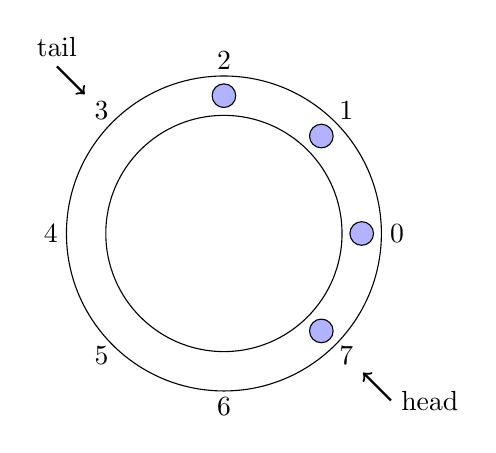
\begin{tikzpicture}
		\draw (0, 0) circle[radius=2];
		\draw (0, 0) circle[radius=1.5];
	
		\foreach \i in {0, 1, 2, 3, 4, 5, 6, 7} {
			\node at ({360/8 * \i}:2.2) {\i};
		}
	
		\foreach \i in {0, 1, 2, 7} {
			\draw[fill=blue!30] ({360/8 * \i}:1.75) circle[radius=0.15];
		}
	
		\draw[->, thick] (-45:3.0) node[right]{head} -- (-45:2.5);
		\draw[->, thick] (135:3.0) node[above]{tail} -- (135:2.5);
	\end{tikzpicture}

	
	% さらに1要素追加:headが進む
	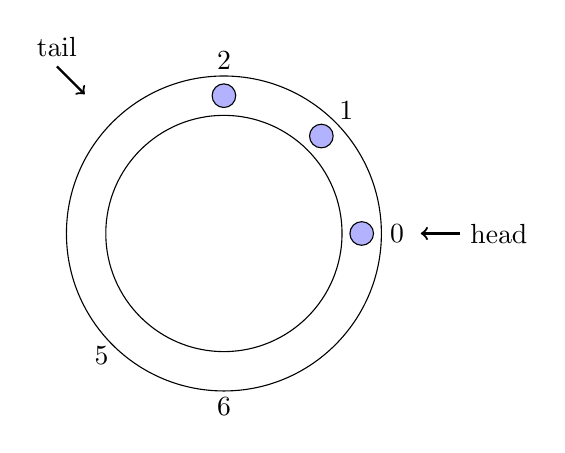
\begin{tikzpicture}
		\draw (0, 0) circle[radius=2];
		\draw (0, 0) circle[radius=1.5];
	
		\foreach \i in {0, 1, 2, 5, 6} {
			\node at ({360/8 * \i}:2.2) {\i};
		}
	
		\foreach \i in {0, 1, 2} {
			\draw[fill=blue!30] ({360/8 * \i}:1.75) circle[radius=0.15];
		}
	
		\draw[->, thick] (0:3.0) node[right]{head} -- (0:2.5);
		\draw[->, thick] (135:3.0) node[above]{tail} -- (135:2.5);
	\end{tikzpicture}
	\end{adjustbox}

\vspace{0.5cm}

\hspace{6cm} \textbf{enqueue()}
\hspace{3cm} \textbf{dequeue()}

リングバッファの仕組みを見てみましょう。enqueueをするときはtailの位置にデータを追加しtailを1だけ進めます。dequeueをするときはheadの位置のデータを取り出しheadを1だけ進めます。headとtailが同じ位置になったときは、キューが空になります。
実装の際は、要素の数で割った余りを使ってheadとtailの位置を管理します。

\subsection{キューの実装}
キューの実装のポイントは以下の3つです。
\begin{itemize}
	\item キューは配列で実装する
	\item 取り出す位置を示すポインタと追加する位置を示すポインタの2つを持つ
	\item リングバッファをモジュロ演算で実装する (\%を使う)
	\item enqueueとdequeueのメソッドを実装する
\end{itemize}

\begin{lstlisting}[caption=キューの実装, frame=TRBL, label={queue}]
	class Queue:
    def __init__(self, size: int) -> None:
        self.queue = [0] * size
        self.size = 0
        self.head = 0
        self.tail = 0
        
    def enqueue(self, value: int) -> None:
        if not self.is_full():
            self.size += 1
            self.queue[self.tail] = value
            self.tail = (self.tail + 1) % len(self.queue)
        else:
            print("queue is full")
    
    def dequeue(self) -> int:
        if not self.is_empty():
            self.size -= 1
            return_value = self.queue[self.head]
            self.head = (self.head + 1) % len(self.queue)
            print(return_value)
        else:
            print("queue is empty")
        
    
    def is_empty(self):
        return self.size == 0

    def is_full(self):
        return self.size == len(self.queue)

queue = Queue(5)

queue.enqueue(8)
queue.enqueue(4)
queue.enqueue(5)

queue.enqueue(2)

queue.dequeue()

\end{lstlisting}

\begin{tcolorbox}[enhanced, title=Column2 collections.deque, breakable, colback=white, drop fuzzy shadow, attach boxed title to top center={yshift*=0.1cm}]
	スタックと同様にキューも実際に使用するときは、Pythonの標準ライブラリであるcollectionsのdequeを使うと便利です。
	
	\begin{lstlisting}[frame=TRBL]
		from collections import deque

queue = deque()

queue.append(8)
queue.append(4)
queue.append(5)

queue.append(2)

return_value = queue.popleft()

print(f"returned value is {return_value}")
	\end{lstlisting}
\end{tcolorbox}

\newpage

\section{線形リスト}

線形リストとは、以下の図のようにデータと次のポインタを持つデータを連結させるデータ構造です。
線形リストは必要なときに必要なデータを追加していくことができるため、空間計算量的に効率がいいです。しかし、データを取り出すときは
先頭から順番にたどる必要があるため、時間計算量的には効率が悪いです。

今回実装する線形リストは以下の操作ができるものです。

\begin{itemize}
	\item 片方向の線形リスト
	\item 新しい要素は常に末尾に追加する
	\item 検索は先頭から順番に行う
\end{itemize}

双方向の線形リストや、データの追加や削除を任意の位置で行うものもありますが、今回は片方向の線形リストを実装します。

\vspace{1cm}

\begin{tikzpicture}[node distance=6cm,baseline=-0.5ex,  arrow/.style = {thick,-stealth}]
    \node(NodeName1){
        \begin{tcolorbox}[width=4cm]
		データ1
		\tcblower
		次へのポインタ
        \end{tcolorbox}
    };
	\node(NodeName2)[right of=NodeName1]{
		\begin{tcolorbox}[width=4cm]
		データ2
		\tcblower
		次へのポインタ
		\end{tcolorbox}
	};
	\node(NodeName3)[right of=NodeName2]{
		\begin{tcolorbox}[width=4cm]
		データ3
		\tcblower
		次へのポインタ
		\end{tcolorbox}
	};

	% 矢印を描画
	\draw[arrow] (NodeName1) -- (NodeName2);
	\draw[arrow] (NodeName2) -- (NodeName3);
\end{tikzpicture}

\vspace{1cm}

\subsection{線形リストの実装}
先ほどのスタックやキューは配列を使って実装しましたが、線形リストはポインタ(Pythonではクラスのインスタンス)を使って要素をつなげて実装します。

\begin{lstlisting}[caption=線形リストの実装, label=linear, frame=TRBL, label={linear}]
class Node:
    def __init__(self, value) -> None:
        self.value = value
        self.next: Node = None
        
class LinkedList:
    def __init__(self) -> None:
        self.head = Node(None)
    
    def append(self, value: int) -> None:
        current_cell = self.head
        while current_cell.next != None:
            current_cell = current_cell.next
        
        # 追加する数値を値にもつノード
        new_cell = Node(value)
        # 現在の最後のノードの次のノードに付け加える
        current_cell.next = new_cell
        
    def pop(self, value: int) -> Node | None:
        """
        valueと同じ数値を値に持つノードを取り除く
        """
        prev_cell = None
        current_cell = self.head
        
        while current_cell != None:
            if current_cell.value == value:
                # 取り出すため、付け替える
                prev_cell.next = current_cell.next
                return value
            else:
                prev_cell = current_cell
                current_cell = current_cell.next
        
        return None

linked_list = LinkedList()

linked_list.append(10)
linked_list.append(535)
linked_list.append(51)
linked_list.append(40)
linked_list.append(40)
linked_list.append(1)

return_value = linked_list.pop(51)

print(return_value)

\end{lstlisting}

\newpage

\section{ツリー(木構造)}
木をひっくり返して根っこを上にして書いた木のような離散構造をツリーと言います。ツリーは用語が重要なため、以下の用語を覚えておくと良いです。

\subsection{木構造の用語}

\subsubsection{根と葉}

一番上のノードを\textbf{根}、一番下のノード(より下に子ノードを持っていないノード)\textbf{葉}といいます。

\vspace{1cm}

\begin{center}
	\begin{tikzpicture}[scale=0.4]
		\node[circle, draw, minimum size=1.2cm] (A) at (0, 0) {};
		\node[circle, draw, minimum size=1.2cm] (B) at (-4, -5) {};
		\node[circle, draw, minimum size=1.2cm] (C) at (4, -5) {};
		\node[circle, draw, minimum size=1.2cm] (D) at (-9, -10) {};
		\node[circle, draw, minimum size=1.2cm] (E) at (-13, -10) {};
		\node[circle, draw, minimum size=1.2cm] (F) at (-2, -10) {};
		\node[circle, draw, minimum size=1.2cm] (G) at (-6, -10) {};
		\node[circle, draw, minimum size=1.2cm] (H) at (2, -10) {};
	
		\draw (A) -- (B);
		\draw (A) -- (C);
		\draw (B) -- (D);
		\draw (B) -- (E);
		\draw (B) -- (F);
		\draw (B) -- (G);
		\draw (C) -- (H);

		% 円の中に文字を入れる
		\node at (0, 0) {根};

		% 葉には葉と書く
		\node at (-9, -10) {葉};
		\node at (-13, -10) {葉};
		\node at (-2, -10) {葉};
		\node at (-6, -10) {葉};
		\node at (2, -10) {葉};
	\end{tikzpicture}
\end{center}


\subsubsection{深さと高さ}

あるノードから繋がっている葉までの自分を除いたノードの数のうち最大の個数を\textbf{高さ}といいます。 葉ノード自体の高さは0です。また、
根からあるノードまでの高さを\textbf{深さ}といいます。

\vspace{1cm}
\begin{center}
	\begin{tikzpicture}[scale=0.4]
		\node[circle, draw, minimum size=1.2cm] (A) at (0, 0) {};
		\node[circle, draw, minimum size=1.2cm] (B) at (-4, -5) {};
		\node[circle, draw, minimum size=1.2cm] (C) at (4, -5) {};
		\node[circle, draw, minimum size=1.2cm] (D) at (-8, -10) {};
		\node[circle, draw, minimum size=1.2cm] (E) at (-0.5, -10) {};
		\node[circle, draw, minimum size=1.2cm] (F) at (-12, -15) {};
	
		\draw (A) -- (B);
		\draw (A) -- (C);
		\draw (B) -- (D);
		\draw (B) -- (E);
		\draw (D) -- (F);

		% 円の中に数字を入れる
		\node at (0, 0) {1};
		\node at (-4, -5) {2};
		\node at (4, -5) {3};
		\node at (-8, -10) {4};
		\node at (-0.5, -10) {5};
		\node at (-12, -15) {6};	

	\end{tikzpicture}
	\end{center}

\subsubsection{二分木(binary tree)}
すべてのノードに関して、その子ノードの数が2以下である木を\textbf{二分木}といいます。二分木は以下のような特徴があります。上の木も
二分木になっています。

また、、完全二分木というものがあります。完全二分技は英語で表記するとfull binary treeとcomplete binary treeがあります。これらは独立した定義ですので、注意してください。
違いを整理すると以下のようになります。

\begin{itemize}
	\item full binary tree: すべてのノードが0個または2個の子ノードを持つ二分木
	\item complete binary tree: 根がある階層(level)を除いて、すべての階層で埋まりうるノードがすべて埋まっているかつ、最後の階層のノードは左から右に向かって埋まっている二分木
\end{itemize}

両者の違いは最初は分かりにくいです、以下の図を見て理解を深めてください。

\vspace{1cm}

\begin{figure}[htbp]
\begin{center}
	\begin{tabular}{cc}
		\begin{tikzpicture}[scale=0.4]
			\node[circle, draw, minimum size=1.2cm] (A) at (0, 0) {};
			\node[circle, draw, minimum size=1.2cm] (B) at (-4, -5) {};
			\node[circle, draw, minimum size=1.2cm] (C) at (4, -5) {};
			\node[circle, draw, minimum size=1.2cm] (D) at (8, -10) {};
			\node[circle, draw, minimum size=1.2cm] (E) at (0, -10) {};

			\draw (A) -- (B);
			\draw (A) -- (C);
			\draw (C) -- (D);
			\draw (C) -- (E);
		\end{tikzpicture}

		& 
		\begin{tikzpicture}[scale=0.4]
			\node[circle, draw, minimum size=1.2cm] (A) at (0, 0) {};
			\node[circle, draw, minimum size=1.2cm] (B) at (-4, -5) {};
			\node[circle, draw, minimum size=1.2cm] (C) at (-6, -10) {};
			\node[circle, draw, minimum size=1.2cm] (D) at (-2, -10) {};
			\node[circle, draw, minimum size=1.2cm] (H) at (-8, -15) {};

			\node[circle, draw, minimum size=1.2cm] (E) at (4, -5) {};
			\node[circle, draw, minimum size=1.2cm] (F) at (8, -10) {};
			\node[circle, draw, minimum size=1.2cm] (G) at (2, -10) {};

			\draw (A) -- (B);
			\draw (B) -- (C);
			\draw (B) -- (D);

			\draw (A) -- (E);
			\draw (E) -- (F);
			\draw (E) -- (G);
			\draw (C) -- (H);

		\end{tikzpicture}
	\end{tabular}
\end{center}
\end{figure}

\hspace{1.5cm} full binary treeの例 \hspace{4.5cm} complete binary treeの例

\newpage

\section{ヒープ}
木構造を使ったデータ構造にヒープがあります。ヒープは以下の特徴があります。

\begin{itemize}
	\item 親ノードは子ノードよりも大きい(または小さい)という性質を持つ
	\item 根ノードは常に最大(または最小)となる
\end{itemize}

さらに今回はヒープの中でさらに、complete binary treeになっている\textbf{二分ヒープ}というデータ構造を扱います。ヒープはcomplete binary tree
に対して、以下の操作を行います。

\begin{itemize}
	\item 要素の追加
	\item 要素の取り出し
\end{itemize}

要素の追加に関して、二分ヒープがcomplete binary treeになっているため、根がある階層(level)の一番右に要素を追加してきます。
追加時に、追加したノードから根までヒープの条件を満たすように再帰的にノードを交換していきます。以下は最小ヒープの例です。

\vspace{1cm}

\begin{figure}[htbp]
	\begin{center}
		\begin{tabular}{cc}
			\begin{tikzpicture}[scale=0.4]
				\node[circle, draw, minimum size=1.2cm] (A) at (0, 0) {};
				\node[circle, draw, minimum size=1.2cm] (B) at (-4, -5) {};
				\node[circle, draw, minimum size=1.2cm] (C) at (4, -5) {};
				\node[circle, draw, minimum size=1.2cm] (D) at (-8, -10) {};
	
				% 線を引く
				\draw (A) -- (B);
				\draw (A) -- (C);
				\draw (B) -- (D);

				% 値を入れる
				\node at (0, 0) {1};
				\node at (-4, -5) {3};
				\node at (4, -5) {4};
				\node at (-8, -10) {6};
			\end{tikzpicture}
			&
			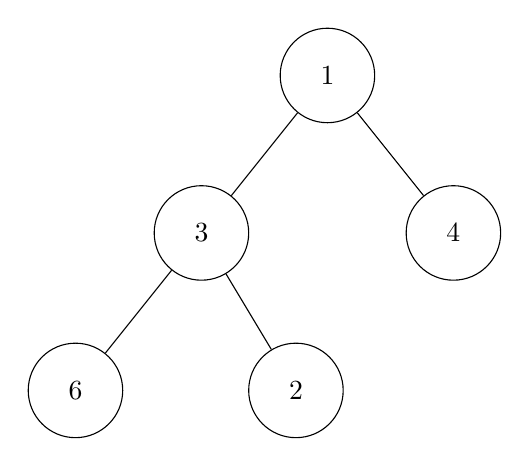
\begin{tikzpicture}[scale=0.4]
				\node[circle, draw, minimum size=1.2cm] (A) at (0, 0) {};
				\node[circle, draw, minimum size=1.2cm] (B) at (-4, -5) {};
				\node[circle, draw, minimum size=1.2cm] (C) at (4, -5) {};
				\node[circle, draw, minimum size=1.2cm] (D) at (-8, -10) {};
				\node[circle, draw, minimum size=1.2cm] (E) at (-1, -10) {};
	
				% 線を引く
				\draw (A) --(B);
				\draw (A) -- (C);
				\draw (B) -- (D);
				\draw (B) -- (E);

				% 値を入れる
				\node at (0, 0) {1};
				\node at (-4, -5) {3};
				\node at (4, -5) {4};
				\node at (-8, -10) {6};
				\node at (-1, -10) {2};
			\end{tikzpicture}
		\end{tabular}
		\begin{tikzpicture}[overlay, scale=0.4]
			\draw[->, thick] (-16, 0) -- (-13, 0);
			\node at (-14.7, -1.8) {追加};
		\end{tikzpicture}
	\end{center}
	\end{figure}

\vspace{1cm}

二分ヒープからの削除は少し複雑です。以下のような操作を行います。

\begin{enumerate}
	\item 根ノードを取り除く
	\item 一番右下のノードを根に移動する
	\item 根から下に向かって、子ノードと比較して、ヒープの条件を満たすように再帰的にノードを交換していく
\end{enumerate}

一番右のノードを根に移動する理由は、complete binary treeを保つためです。もしも、根を取り除いた後に直接根の子ノード
を根にしてしまうと、必ずしもcomplete binary treeにならず実装が複雑になります。

\begin{figure}[htbp]
	\begin{center}
		\begin{tabular}{cc}
			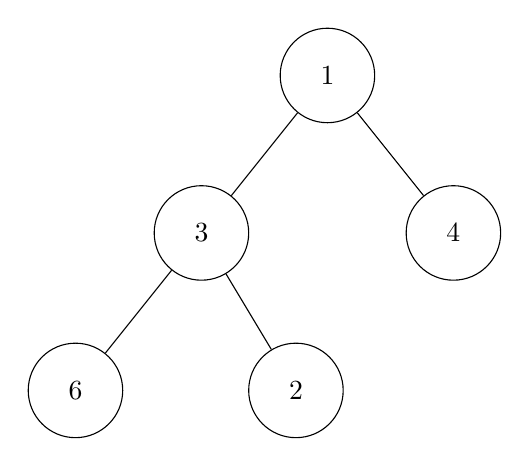
\begin{tikzpicture}[scale=0.4]
				\node[circle, draw, minimum size=1.2cm] (A) at (0, 0) {};
				\node[circle, draw, minimum size=1.2cm] (B) at (-4, -5) {};
				\node[circle, draw, minimum size=1.2cm] (C) at (4, -5) {};
				\node[circle, draw, minimum size=1.2cm] (D) at (-8, -10) {};
				\node[circle, draw, minimum size=1.2cm] (E) at (-1, -10) {};
	
				% 線を引く
				\draw (A) -- (B);
				\draw (A) -- (C);
				\draw (B) -- (D);
				\draw (B) -- (E);

				% 値を入れる
				\node at (0, 0) {1};
				\node at (-4, -5) {3};
				\node at (4, -5) {4};
				\node at (-8, -10) {6};
				\node at (-1, -10) {2};
			\end{tikzpicture}
			&
			\begin{tikzpicture}[scale=0.4]
				\node[circle, draw, minimum size=1.2cm, dashed] (A) at (0, 0) {};
				\node[circle, draw, minimum size=1.2cm] (B) at (-4, -5) {};
				\node[circle, draw, minimum size=1.2cm] (C) at (4, -5) {};
				\node[circle, draw, minimum size=1.2cm] (D) at (-8, -10) {};
				\node[circle, draw, minimum size=1.2cm] (E) at (-1, -10) {};
	
				% 線を引く
				\draw (A) --(B);
				\draw (A) -- (C);
				\draw (B) -- (D);
				\draw (B) -- (E);

				% 値を入れる
				\node at (-4, -5) {3};	
				\node at (4, -5) {4};
				\node at (-8, -10) {6};
				\node at (-1, -10) {2};
				
			\end{tikzpicture}
		\end{tabular}
		\begin{tikzpicture}[overlay, scale=0.4]
			\draw[->, thick] (-16, 0) -- (-13, 0);
			\node at (-14.7, -1.8) {1.根を除く};
		\end{tikzpicture}
	\end{center}
	\end{figure}


\begin{figure}[htbp]
	\begin{center}
		\begin{tabular}{cc}
			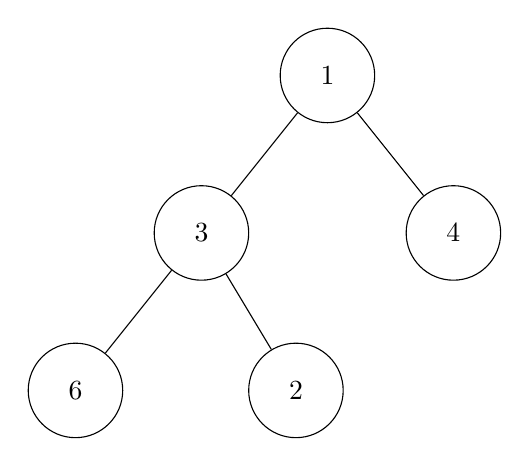
\begin{tikzpicture}[scale=0.4]
				\node[circle, draw, minimum size=1.2cm] (A) at (0, 0) {};
				\node[circle, draw, minimum size=1.2cm] (B) at (-4, -5) {};
				\node[circle, draw, minimum size=1.2cm] (C) at (4, -5) {};
				\node[circle, draw, minimum size=1.2cm] (D) at (-8, -10) {};
				\node[circle, draw, minimum size=1.2cm] (E) at (-1, -10) {};
	
				% 線を引く
				\draw (A) -- (B);
				\draw (A) -- (C);
				\draw (B) -- (D);
				\draw (B) -- (E);

				% 値を入れる
				\node at (0, 0) {1};
				\node at (-4, -5) {3};
				\node at (4, -5) {4};
				\node at (-8, -10) {6};
				\node at (-1, -10) {2};
			\end{tikzpicture}
			&
			\begin{tikzpicture}[scale=0.4]
				\node[circle, draw, minimum size=1.2cm] (A) at (0, 0) {};
				\node[circle, draw, minimum size=1.2cm] (B) at (-4, -5) {};
				\node[circle, draw, minimum size=1.2cm] (C) at (4, -5) {};
				\node[circle, draw, minimum size=1.2cm] (D) at (-8, -10) {};
	
				% 線を引く
				\draw (A) --(B);
				\draw (A) -- (C);
				\draw (B) -- (D);

				% 値を入れる
				\node at (0, 0) {2};
				\node at (-4, -5) {3};	
				\node at (4, -5) {4};
				\node at (-8, -10) {6};
				
			\end{tikzpicture}
		\end{tabular}
		\begin{tikzpicture}[overlay, scale=0.4]
			\draw[->, thick] (-16, 0) -- (-13, 0);
			\node at (-14.7, -1.8) {2.右下を根に};
		\end{tikzpicture}
	\end{center}
	\end{figure}

上の例では、根を取り除き一番右のノードを根に移動すると木がヒープの性質を満たしていますが、一般的にはヒープの性質を満たすまで
根から下に向かってノードを再帰的に交換していきます。

\subsection{ヒープの実装}
二分ヒープの実装のポイントは

\begin{itemize}
	\item 1-indexedの配列で実装する(要素数 + 1の大きさの配列を用意する)
\end{itemize}


二分木は構造体を使わず配列だけで実装できる点が利点です。以下は最小ヒープの実装です。

\begin{lstlisting}[caption=二分ヒープの実装, label=binaryheap, frame=TRBL, label={binaryheap}]
class Heap:
	def __init__(self, size: int) -> None:
		self.inf = 1 << 60
		self.size = size + 1
		self.heap = [self.inf] * self.size
		self.tail = 0 # 現在のヒープのデータ数
		
	# 複数回swap処理が登場するためメソッドにした
	def swap(self, index1: int, index2: int) -> None:
		self.heap[index1], self.heap[index2] = self.heap[index2], self.heap[index1]

	def push(self, value: int) -> None:
		if self.tail != self.size - 1:
			self.tail += 1
			self.heap[self.tail] = value
			self.check_from_leaf(self.tail)

	def check_from_leaf(self, node: int) -> None:
		# nodeが根なら再帰終了
		if node == 1:
			return
		
		parent = node // 2
		# ヒープの条件を満たさない
		if self.heap[parent] > self.heap[node]:
			self.swap(parent, node)
			self.check_from_leaf(parent)
		

	def pop(self) -> int | None:
		if self.tail != 0:
			popping_value = self.heap[1]
			# 一番右の葉ノードを根ノードに移動
			self.heap[1] = self.heap[self.tail]
			self.tail -= 1
			self.check_from_root(1)
			return popping_value
		else:
			return None

	def check_from_root(self, node: int) -> None:
		left_child, right_child = 2 * node, 2 * node + 1
		
		# left > rightよりこれだけで十分
		if left_child > self.tail:
			return
		
		# 2つの子ノードの大小で区別する
		smaller_node = larger_node = 0
		if self.heap[left_child] < self.heap[right_child]:
			smaller_node, larger_node = left_child, right_child
		else:
			smaller_node, larger_node = right_child, left_child
		
		# 親ノードと小さい方の子ノードを比較
		if self.heap[node] > self.heap[smaller_node]:
			self.swap(node, smaller_node)
			# 小さい方だけで十分
			self.check_from_root(smaller_node)

\end{lstlisting}

\newpage

\section{セグメント木}
セグメント木はある条件を満たす演算に関する区間の計算結果を高速に求めるデータ構造です。区間の計算結果を高速にもとめると聞いて
累積和や尺取法を思い浮かべるかもしれませんが、セグメント木は扱うデータの要素が逐一変わるような状況でも区間の計算結果を高速に求めることができます。
具体的な演算は、区間の最大・最小値や、合計値などがあります。

\subsection{数学の知識の確認}
セグメント木の内容に入る前に、セグメント木を理解するのに必要な数学の知識を整理します。

\subsubsection{二項演算}

自然数や文字列の集合$S$の任意2つの元から新たに値を生成する操作のことを\textbf{$S$上の二項演算}といいます。
特に、$x, y \in S$に対する二項演算を$op(x, y)$と書き、

% equation*とすると、数式の番号がつかなくなる. 
\begin{equation*}
	op(x, y) = x * y
\end{equation*}

と表現することにします。

\subsubsection{閉じた演算}
$x, y \in S$に対して$op(x, y) \in S$を満たすような演算を閉じた演算といいます。例えば、自然数の集合$S$において、
$op(x, y) = x + y$は閉じた演算ですが、$op(x, y) = x - y$は閉じた演算ではありません。

今回実装するセグメント木は、閉じた演算を扱うため、セグメント木の演算は閉じた演算になるようにします。

\subsubsection{完全二分木}
セグメント木は完全二分木になっています。以下の図のように根以外のすべてのノードが2つの子ノードを持っていて、すべての葉の深さが同じ木になっています。

\vspace{0.25cm}

\begin{center}
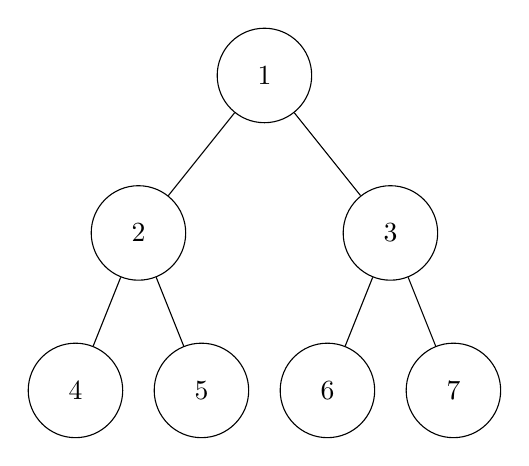
\begin{tikzpicture}[scale=0.4]
    % ノードを描画
    \node[circle, draw, minimum size=1.2cm] (A) at (0, 0) {1};
    \node[circle, draw, minimum size=1.2cm] (B) at (-4, -5) {2};
    \node[circle, draw, minimum size=1.2cm] (C) at (4, -5) {3};
    \node[circle, draw, minimum size=1.2cm] (D) at (-6, -10) {4};
    \node[circle, draw, minimum size=1.2cm] (E) at (-2, -10) {5};
    \node[circle, draw, minimum size=1.2cm] (F) at (2, -10) {6};
    \node[circle, draw, minimum size=1.2cm] (G) at (6, -10) {7};

    % エッジを描画
    \draw (A) -- (B);
    \draw (A) -- (C);
    \draw (B) -- (D);
    \draw (B) -- (E);
    \draw (C) -- (F);
    \draw (C) -- (G);
\end{tikzpicture}
\end{center}

\subsection{セグメント木の仕組み}

セグメント木の理解に必要な知識の整理が終わったので、セグメント木の内容に入ります。

\subsubsection{セグメント木の構造}
セグメント木の構造の特徴は以下の通りです。下の図は$a_0からa_6$の7個のデータを持つセグメント木の例です。

\begin{itemize}
	\item 葉ノードにデータを持つ
	\item 親ノードは2つの子ノードの演算結果を持つ
	\item $op(x, y)$は結合法則を満たす ($(x * y) * z = x * (y * z)$が成立する)
	\item 集合$S$に対する$op$に単位元が存在する
\end{itemize}

\vspace{1cm}

\begin{center}
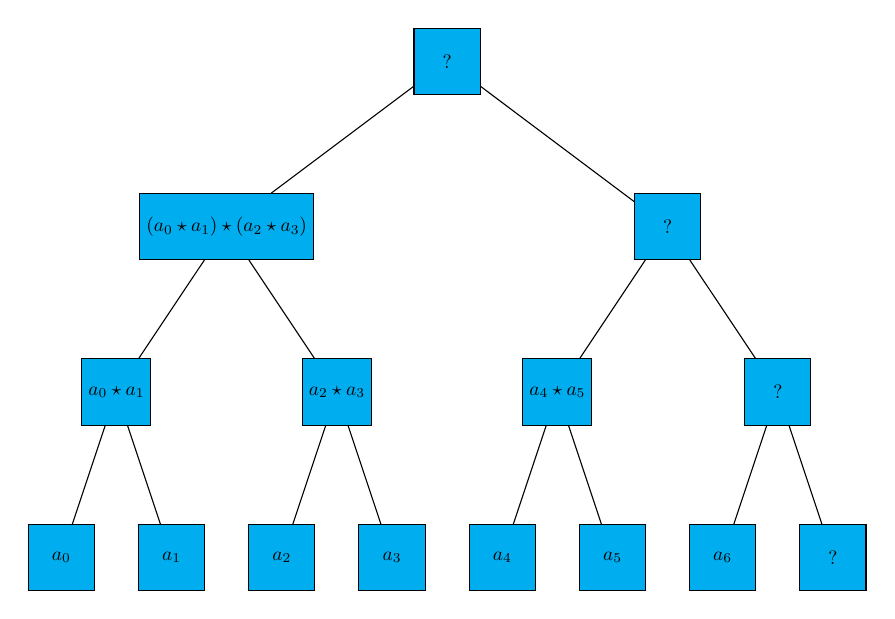
\begin{tikzpicture}[scale=0.7, transform shape]
    % ノードを描画
    \node[draw, rectangle, fill=cyan, minimum size=1.2cm] (A) at (0, 0) {?};
    \node[draw, rectangle, fill=cyan, minimum size=1.2cm] (B) at (-4, -3) {$(a_0 \star a_1) \star (a_2 \star a_3)$};
    \node[draw, rectangle, fill=cyan, minimum size=1.2cm] (C) at (4, -3) {?};
    \node[draw, rectangle, fill=cyan, minimum size=1.2cm] (D) at (-6, -6) {$a_0 \star a_1$};
    \node[draw, rectangle, fill=cyan, minimum size=1.2cm] (E) at (-2, -6) {$a_2 \star a_3$};
    \node[draw, rectangle, fill=cyan, minimum size=1.2cm] (F) at (2, -6) {$a_4 \star a_5$};
    \node[draw, rectangle, fill=cyan, minimum size=1.2cm] (G) at (6, -6) {?};
    \node[draw, rectangle, fill=cyan, minimum size=1.2cm] (H) at (-7, -9) {$a_0$};
    \node[draw, rectangle, fill=cyan, minimum size=1.2cm] (I) at (-5, -9) {$a_1$};
    \node[draw, rectangle, fill=cyan, minimum size=1.2cm] (J) at (-3, -9) {$a_2$};
    \node[draw, rectangle, fill=cyan, minimum size=1.2cm] (K) at (-1, -9) {$a_3$};
    \node[draw, rectangle, fill=cyan, minimum size=1.2cm] (L) at (1, -9) {$a_4$};
    \node[draw, rectangle, fill=cyan, minimum size=1.2cm] (M) at (3, -9) {$a_5$};
    \node[draw, rectangle, fill=cyan, minimum size=1.2cm] (N) at (5, -9) {$a_6$};
    \node[draw, rectangle, fill=cyan, minimum size=1.2cm] (O) at (7, -9) {?};

    % エッジを描画
    \draw (A) -- (B);
    \draw (A) -- (C);
    \draw (B) -- (D);
    \draw (B) -- (E);
    \draw (C) -- (F);
    \draw (C) -- (G);
    \draw (D) -- (H);
    \draw (D) -- (I);
    \draw (E) -- (J);
    \draw (E) -- (K);
    \draw (F) -- (L);
    \draw (F) -- (M);
    \draw (G) -- (N);
    \draw (G) -- (O);
\end{tikzpicture}
\end{center}

\vspace{1cm}

図には?があります。?を\textbf{全要素の総積をセグメント木の根が持つ}ように埋めていきます。下の図の$e$は単位元を表しています。
根$a_0 * a_1 * a_2 * a_3 * a_4 * a_5 * a_6$は全要素の総積になっていることを考えると、その下の?
は$a_4 * a_5 * a_6$になります。同様に、そのほかの?も埋めていくと以下の図のようになります。

\vspace{1cm}


\begin{center}
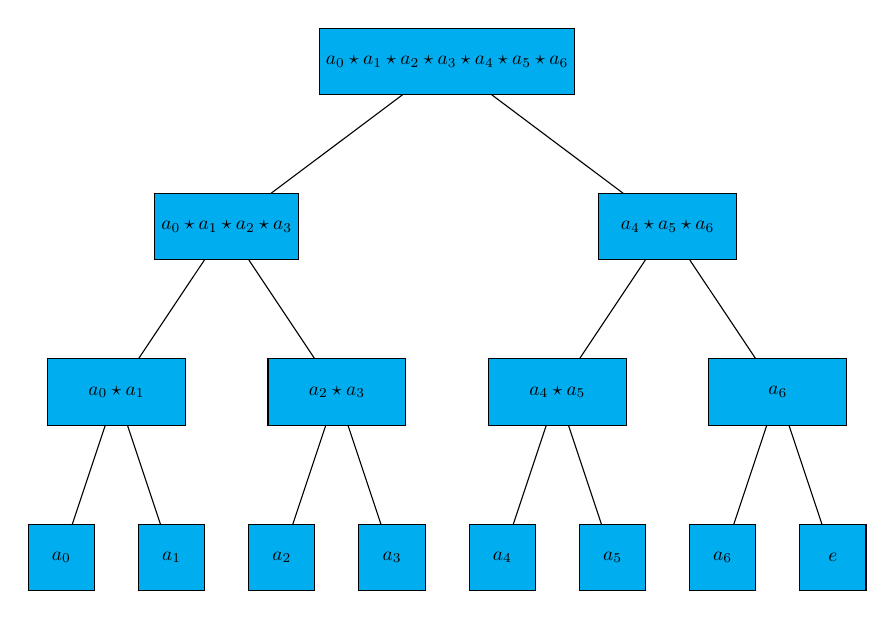
\begin{tikzpicture}[scale=0.7, transform shape]
    % ノードを描画
    \node[draw, rectangle, fill=cyan, minimum width=2.5cm, minimum height=1.2cm] (A) at (0, 0) {$a_0 \star a_1 \star a_2 \star a_3 \star a_4 \star a_5 \star a_6$};
    \node[draw, rectangle, fill=cyan, minimum width=2.5cm, minimum height=1.2cm] (B) at (-4, -3) {$a_0 \star a_1 \star a_2 \star a_3$};
    \node[draw, rectangle, fill=cyan, minimum width=2.5cm, minimum height=1.2cm] (C) at (4, -3) {$a_4 \star a_5 \star a_6$};
    \node[draw, rectangle, fill=cyan, minimum width=2.5cm, minimum height=1.2cm] (D) at (-6, -6) {$a_0 \star a_1$};
    \node[draw, rectangle, fill=cyan, minimum width=2.5cm, minimum height=1.2cm] (E) at (-2, -6) {$a_2 \star a_3$};
    \node[draw, rectangle, fill=cyan, minimum width=2.5cm, minimum height=1.2cm] (F) at (2, -6) {$a_4 \star a_5$};
    \node[draw, rectangle, fill=cyan, minimum width=2.5cm, minimum height=1.2cm] (G) at (6, -6) {$a_6$};
    \node[draw, rectangle, fill=cyan, minimum width=1.2cm, minimum height=1.2cm] (H) at (-7, -9) {$a_0$};
    \node[draw, rectangle, fill=cyan, minimum width=1.2cm, minimum height=1.2cm] (I) at (-5, -9) {$a_1$};
    \node[draw, rectangle, fill=cyan, minimum width=1.2cm, minimum height=1.2cm] (J) at (-3, -9) {$a_2$};
    \node[draw, rectangle, fill=cyan, minimum width=1.2cm, minimum height=1.2cm] (K) at (-1, -9) {$a_3$};
    \node[draw, rectangle, fill=cyan, minimum width=1.2cm, minimum height=1.2cm] (L) at (1, -9) {$a_4$};
    \node[draw, rectangle, fill=cyan, minimum width=1.2cm, minimum height=1.2cm] (M) at (3, -9) {$a_5$};
    \node[draw, rectangle, fill=cyan, minimum width=1.2cm, minimum height=1.2cm] (N) at (5, -9) {$a_6$};
    \node[draw, rectangle, fill=cyan, minimum width=1.2cm, minimum height=1.2cm] (O) at (7, -9) {$e$};

    % エッジを描画
    \draw (A) -- (B);
    \draw (A) -- (C);
    \draw (B) -- (D);
    \draw (B) -- (E);
    \draw (C) -- (F);
    \draw (C) -- (G);
    \draw (D) -- (H);
    \draw (D) -- (I);
    \draw (E) -- (J);
    \draw (E) -- (K);
    \draw (F) -- (L);
    \draw (F) -- (M);
    \draw (G) -- (N);
    \draw (G) -- (O);
\end{tikzpicture}
\end{center}

\vspace{1cm}

\subsection{セグメント木の実装}
セグメント木も二分木なので配列で表現することが可能です。ヒープと同様に1-indexedで実装します。以下の操作ができるようなセグメント木
を実装します。

\begin{itemize}
	\item セグメント木の構築
	\item 要素の更新
	\item 区間の演算結果の取得
\end{itemize}

\subsubsection{セグメント木の構築}
セグメント木では葉にデータが格納され、葉の数はデータの数以上でかつ$2^m$で表せられる最小の数になります。$2^m$は2進数表記にすると$2^m = 1\underbrace{00\cdots0}_{m}$となるので、2進数表記したときにm桁になる数と
$2^m$になる数であるときは葉の数を$2^m$にします。つまり、データの数$n$が$2^{m-1} + 1 \leq n \leq 2^m$であるとき、葉の数は$2^m$になります。そして今回のセグメント木は1-indexedのedの木になっているため配列の0番目の
要素は無視します。よって、配列全体の長さは$2 m$個になります。

セグメント木では扱う演算についての単位元を用意する必要があります。例えば、区間の最大値を求めるセグメント木では、単位元は$-\infty$になります。区間和では単位元は0になります。

葉をデータと単位元で埋めたら、その他のノードは2つの子ノードのデータを使って更新していきます。

\subsubsection{要素の更新}
更新クエリに対しては、該当する葉ノードを更新した後、その親ノードを更新していきます。

\subsubsection{区間の演算結果の取得}
区間の演算結果の取得は少々複雑です。何個か例を挙げて説明します。右開区間[left, right)の区間の演算結果を求めてみます。下のセグメント木を例にします。ノードの近くの数字は1-indexedな配列でセグメント木を表現し
したときのインデックス番号です。

・$left = 0, right = 3$のとき

求めるものは$a_0 * a_1 * a_2 = (a_0 * a_1) * a_1$つまり4と10の演算結果になります。 

・ $left = 1, right = 7$のとき

求めるものは$a_0 * a_1 * a_2 * a_3 * a_4 * a_5 * a_6 = a_1 * (a_2 * a_3) * (a_4 * a_5) * a_6$つまり、9と5と6と14の演算結果になります。

\vspace{1cm}

\begin{center}
	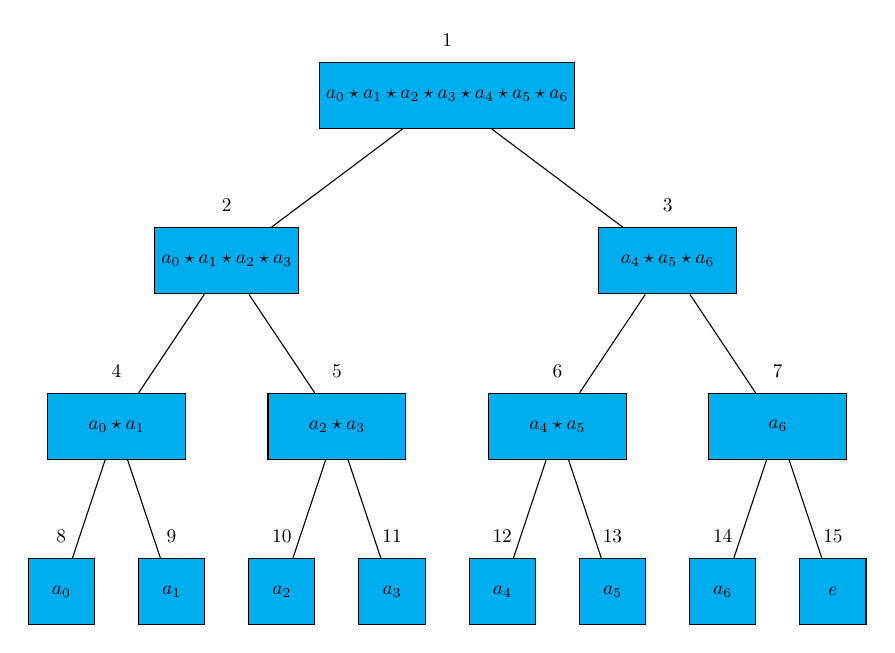
\begin{tikzpicture}[scale=0.7, transform shape]
		% ノードを描画
		\node[draw, rectangle, fill=cyan, minimum width=2.5cm, minimum height=1.2cm] (A) at (0, 0) {$a_0 \star a_1 \star a_2 \star a_3 \star a_4 \star a_5 \star a_6$};
		\node[draw, rectangle, fill=cyan, minimum width=2.5cm, minimum height=1.2cm] (B) at (-4, -3) {$a_0 \star a_1 \star a_2 \star a_3$};
		\node[draw, rectangle, fill=cyan, minimum width=2.5cm, minimum height=1.2cm] (C) at (4, -3) {$a_4 \star a_5 \star a_6$};
		\node[draw, rectangle, fill=cyan, minimum width=2.5cm, minimum height=1.2cm] (D) at (-6, -6) {$a_0 \star a_1$};
		\node[draw, rectangle, fill=cyan, minimum width=2.5cm, minimum height=1.2cm] (E) at (-2, -6) {$a_2 \star a_3$};
		\node[draw, rectangle, fill=cyan, minimum width=2.5cm, minimum height=1.2cm] (F) at (2, -6) {$a_4 \star a_5$};
		\node[draw, rectangle, fill=cyan, minimum width=2.5cm, minimum height=1.2cm] (G) at (6, -6) {$a_6$};
		\node[draw, rectangle, fill=cyan, minimum width=1.2cm, minimum height=1.2cm] (H) at (-7, -9) {$a_0$};
		\node[draw, rectangle, fill=cyan, minimum width=1.2cm, minimum height=1.2cm] (I) at (-5, -9) {$a_1$};
		\node[draw, rectangle, fill=cyan, minimum width=1.2cm, minimum height=1.2cm] (J) at (-3, -9) {$a_2$};
		\node[draw, rectangle, fill=cyan, minimum width=1.2cm, minimum height=1.2cm] (K) at (-1, -9) {$a_3$};
		\node[draw, rectangle, fill=cyan, minimum width=1.2cm, minimum height=1.2cm] (L) at (1, -9) {$a_4$};
		\node[draw, rectangle, fill=cyan, minimum width=1.2cm, minimum height=1.2cm] (M) at (3, -9) {$a_5$};
		\node[draw, rectangle, fill=cyan, minimum width=1.2cm, minimum height=1.2cm] (N) at (5, -9) {$a_6$};
		\node[draw, rectangle, fill=cyan, minimum width=1.2cm, minimum height=1.2cm] (O) at (7, -9) {$e$};
	
		% インデックス番号を追加
		\node at (0, 1) {1};
		\node at (-4, -2) {2};
		\node at (4, -2) {3};
		\node at (-6, -5) {4};
		\node at (-2, -5) {5};
		\node at (2, -5) {6};
		\node at (6, -5) {7};
		\node at (-7, -8) {8};
		\node at (-5, -8) {9};
		\node at (-3, -8) {10};
		\node at (-1, -8) {11};
		\node at (1, -8) {12};
		\node at (3, -8) {13};
		\node at (5, -8) {14};
		\node at (7, -8) {15};
	
		% エッジを描画
		\draw (A) -- (B);
		\draw (A) -- (C);
		\draw (B) -- (D);
		\draw (B) -- (E);
		\draw (C) -- (F);
		\draw (C) -- (G);
		\draw (D) -- (H);
		\draw (D) -- (I);
		\draw (E) -- (J);
		\draw (E) -- (K);
		\draw (F) -- (L);
		\draw (F) -- (M);
		\draw (G) -- (N);
		\draw (G) -- (O);
	\end{tikzpicture}
\end{center}

\vspace{1cm}

どのノードを使うかを機械的に判断していくにはどうすればいいでしょうか。それは、$left$と$right$が親ノードから見て右子ノードか左子ノードにあるかを見ていけばいいです。
leftとrightが右か左にあるかを見ていき、両者の間隔を狭めていって、leftとrightが同じノードになるまで続けます。

1. leftを右に移動する

leftが指すノードを使うか、それともその親ノードを使うかの判定を考えます。leftとrightの間は連続した区間であることに注意すると、leftが親の左側にある場合は親ノードの値を使えばいいことがわかります。
一方で、leftが親の右側にある場合は、leftが指すノードの値を使う必要があります。また1-indexedなセグメント木では右ノードと左ノードは偶奇で判定できます。

2. rightを左に移動する

rightも同様に考えます。ただ、rightは開区間になっているためright - 1を使うか使わないかを考えます。rightが親の左側にある時はright - 1よりも左側の要素を使うことになりますが、それはright - 1の親ノード
が含んでいるため、right - 1は使いません。一方、rightが親の右側にある場合はright - 1を使う必要があります。

\subsubsection{実装}

以上の考察をコードにします。以下は区間の最大値を求めるセグメント木の実装例です。


\begin{lstlisting}[caption=セグメント木の実装, label=segment, frame=TRBL, label={segment}]
# 区間の最大値を求めるセグメント木
class SegmentTree:
    def __init__(self, data_size: int, v: list[int] | None = None):
        self.data_size = data_size
        self.log = (data_size - 1).bit_length()
        self.capacity = 1 << self.log
        self.e = - (1 << 60)
        self.tree = [self.e] * (2 * self.capacity)

        # データが事前に与えられている場合
        if v is not None:
            # 葉ノードを埋める
            for i in range(self.data_size):
                 self.tree[self.capacity + i] = v[i]
                 
            # 葉ノード以外を埋める 
            for i in range(self.capacity - 1, 0, -1):
                self.update(i)
    
    def update(self, index: int) -> None:
        self.tree[index] = max(self.tree[2 * index], self.tree[2 * index + 1])

    # 更新クエリ
    def set(self, index: int, value: int) -> None:
        # 葉に移動
        index += self.capacity
        # 更新
        self.tree[index] = value
        # 上のノードを更新 根(1)を更新するまで続ける
        while index > 1:
            index //= 2
            self._update(index)
            
    # 取得クエリ
    def prod(self, left: int, right: int) -> int:
        left_value = right_value = self.e
        
        # 葉に移動
        left += self.capacity
        right += self.capacity
        
        while left < right:
            # 範囲の左側が右のノード、本実装では奇数
            if left % 2 == 1:
                left_value = max(left_value, self.tree[left])
                left += 1
            
            if right & 2 == 1:
                right -= 1
                right_value = max(right_value, self.tree[right])
                
            # 親に移動
            left //= 2 
            right //= 2
        
        return max(left_value, right_value)

    def all_prod(self):
        return self.tree[1]
    

\end{lstlisting}

\newpage

\section{BIT}
BIT(Binary Indexed Tree)はフェニック木とも呼ばれるデータ構造で、要素の値が変化する区間の\textbf{和}を高速に求めることができます。
セグメント木でも区間和の計算ができますが、BITはセグメント木よりもシンプルに実装が可能です。区間和に限定すればセグメント木は牛刀をもって鶏を割く
ようなものです。セグメント木はより一般的な演算に対応したデータ構造です。

BITはセグメント木に比べてシンプルです。

\subsection{和}

1番目からi番目の要素の和を高速に求めるために、以下のような操作を行います。

\begin{enumerate}
	\item iを2進数表記にしたときに一番右にある1の要素を足していく
	\item 1の要素を足していくときに、その要素を取り除いて次の1の要素を足していく
\end{enumerate}

例えば、$i = 7$の場合を考えると、$7 = 111(2)$となり、右から1を引いていくと、$111(2), 110(2), 100(2), 000(2)$、つまり$7, 6, 4, 0$となります。

BITのデータを持つ配列をbitとすると、1から7番目の要素の和は、bit[0] = 0になっているので、
\begin{equation*}
	\text{bit}[7] + \text{bit}[6] + \text{bit}[4] + \text{bit}[0]
\end{equation*}

になります。

\subsection{更新}

要素の更新は和の計算と逆の操作を行います。具体的には、以下の操作を行います。

\begin{enumerate}
	\item iを2進数表記にしたときに一番右にある1の要素を引いていく
	\item 1の要素を引いていくときに、その要素を取り除いて次の1の要素を引いていく
\end{enumerate}

例えば、$A = [1, 2, 3, 4, 5, 6, 7, 8]$という等差数列の5番目に6を足すと、$A = [1, 2, 3, 4, 11, 6, 7, 8]$になります。このような値の更新をBITで行ってみましょう。

まず、5を2進数で表すと、$101_2$となります。ここで、一番右にある1の桁に1を足す操作を順に行っていきます。$N = 8$を超える前に操作をやめます。

具体的には、$101_2 \rightarrow 110_2 \rightarrow 1000_2$ となります。これを10進数に直すと、5→6→8となります。ここで出てきた数をインデックスとして、6を足していくことで値を更新することができます。

実際の操作は以下のようになります。

\begin{verbatim}
BIT[5] += 6
BIT[6] += 6
BIT[8] += 6
\end{verbatim}

\subsection{実装}
BITの実装例は以下の通りです。

\begin{lstlisting}[caption=BITの実装, label=bit, frame=TRBL, label={bit}]
	class BIT:
    def __init__(self, size: int) -> None:
        self.size = size
        self.tree = [0] * (size + 1)
    
    def sum(self, index: int) -> int:
        res = 0
        while index > 0:
            res += self.tree[index]
            index -= index & (~index + 1)
        
        return res
    
    def update(self, index: int, value: int) -> None:
        while index < self.size:
            self.tree[index] += value
						index += index & (~index + 1)
\end{lstlisting}

\end{document}

